\documentclass[10pt]{article}
\usepackage[usenames]{color} %used for font color
\usepackage{amssymb} %maths
\usepackage{amsmath} %maths
\usepackage[utf8]{inputenc} %useful to type directly diacritic characters
\usepackage{tikz}
\usetikzlibrary{arrows,positioning,decorations.pathreplacing} \begin{document}
\[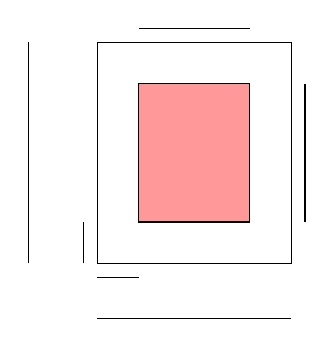
\begin{tikzpicture}
%
\node[draw=black,minimum width=7em,minimum height=8em,rectangle]  at (0,0) {};
\node[draw=black,fill=red!40,minimum width=4em,minimum height=5em,rectangle]  at (0,0) {};
%
%\node[]  at (-3em,0) {$z$};
%
\draw[] (-4em,-4em) -- (-4em,-2.5em);
\draw[] (-6em,-4em) -- (-6em,4em);
\draw[] (-3.5em,-4.5em) -- (-2em,-4.5em);
\draw[] (-3.5em,-6em) -- (3.5em,-6em);
%
\draw[] (4em,-2.5em) -- (4em,2.5em);
\draw[] (-2em,4.5em) -- (2em,4.5em);
%\draw [decorate,decoration={brace}] (0,5em) -- (0,-5em) node [black,midway] {};
\end{tikzpicture}
\\\\
\footnotesize{{\sf pml \;\; n \;\; m \;\; nx \;\; ny \;\; pis \;\; pie \;\; pjs \;\; pje}}\]
\end{document}